\documentclass[conference]{acmsiggraph}

\title{A review on crowd simulation and rendering}

\author{Garoe Dorta-Perez}
\pdfauthor{Garoe Dorta-Perez}

\begin{document}

\maketitle

\begin{abstract}

Crowd simulation and rendering has been an active research area for 
X years.

Citations can be done this way~\cite{Aubel2000}.

\end{abstract}


%% Required for all content. 

\section{Introduction}

Crowd simulation and rendering has been an active research area for 
X years!!INCLUDE CITATION!!!. A crowd is much more than the collections of individuals
that form it. And as such the behaviour of the individuals could be
affected by other members of the crowd. As the numbers in the crowd
increase, the interrelations become quite computationally expensive.

The problem to be tackled has actually several differentiated areas. Firstly
there is a \textit{crowd generation problem}, as the modeller this easy to
use tools in order to set up a scene in which a crowd is present. Secondly,
the crowd is a evolving entity so there are \textit{crowd dynamics} to model,
that will govern the state of the crowd over time. Thirdly, the model should
be presented to the user, so a \textit{rendering} stage is needed.

The same tendency is observed on the rendering area. The first approach
was the introduction of LOD !!INCLUDE CITATION!!!. 

\section{Classification}

As a general classification there are two main areas: real-time simulation
and non real-time simulation.

\subsection{Modelling Classifications}

In order to simulate crowd behaviour a number of approaches have been
proposed. As they shared certain similarities they can be divided 
using a common criteria such as time of the simulation and size
of the modelled crowd. So, in the time
axis we have short-term simulations, medium-term simulations and
long-term simulations. While in the size axis there are small,
medium and big size crowds. We can also use criteria according to
the type of model used for the agents in the crowd.

For small and medium crowds \textit{agent based} or \textit{entity based} systems are
commonly used. While for big size crowds the sheer number of individuals
makes it impractical, so the preferred method is to use \textit{flow based}
simulations.

\subsection{Rendering Classifications}

The different types of rendering techniques can be classified in the 
following groups. LOD techniques, impostors, mesh decimation,
mesh subdivision, cloth simulation.

\begin{equation}
 \sum_{j=1}^{z} j = \frac{z(z+1)}{2}
\end{equation}

\begin{eqnarray}
x & \ll & y_{1} + \cdots + y_{n} \\
  & \leq & z
\end{eqnarray}

\section{Mayor milestones}

With the advent of programmable GPU there has been a shift of
general computation from the CPU to the GPU with substantial
increases in performance.

\subsection{Modelling milestones}

\subsection{Rendering milestones}

In order to lower the rendering cost ~\cite{pratt1997humans} TODO CHANGE TO CITED BY OTHER AUTHOR taken from ~\cite{Aubel1999} used a
LOD technique to be able to render crowds, however even though it 
achieved real time performance the realism of the models was quite
poor.


\begin{figure}[ht]
  \centering
  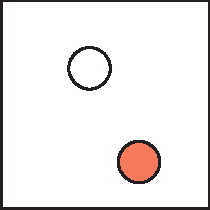
\includegraphics[width=1.5in]{images/samplefigure}
  \caption{Sample illustration.}
\end{figure}
Lorem ipsum dolor sit amet, consectetur adipisicing elit, sed do
eiusmod tempor incididunt ut labore et dolore magna aliqua. Ut enim ad
minim veniam, quis nostrud exercitation ullamco laboris nisi ut
aliquip ex ea commodo consequat. Duis aute irure dolor in
reprehenderit in voluptate velit esse cillum dolore eu fugiat nulla
pariatur. Excepteur sint occaecat cupidatat non proident, sunt in
culpa qui officia deserunt mollit anim id est laborum.

\section{Latest advances}

\subsection{Modelling advances}

\subsection{Rendering advances}

Lorem ipsum dolor sit amet, consectetur adipisicing elit, sed do
eiusmod tempor incididunt ut labore et dolore magna aliqua. Ut enim ad
minim veniam, quis nostrud exercitation ullamco laboris nisi ut
aliquip ex ea commodo consequat. Duis aute irure dolor in
reprehenderit in voluptate velit esse cillum dolore eu fugiat nulla
pariatur. Excepteur sint occaecat cupidatat non proident, sunt in
culpa qui officia deserunt mollit anim id est laborum.

\section{Conclusion}

Lorem ipsum dolor sit amet, consectetur adipisicing elit, sed do
eiusmod tempor incididunt ut labore et dolore magna aliqua. Ut enim ad
minim veniam, quis nostrud exercitation ullamco laboris nisi ut
aliquip ex ea commodo consequat. Duis aute irure dolor in
reprehenderit in voluptate velit esse cillum dolore eu fugiat nulla
pariatur. Excepteur sint occaecat cupidatat non proident, sunt in
culpa qui officia deserunt mollit anim id est laborum.

\section*{Acknowledgements}

To Robert, for all the bagels.

\bibliographystyle{acmsiggraph}
\bibliography{template}
\end{document}
